% Created by tikzDevice version 0.12 on 2018-09-26 16:24:02
% !TEX encoding = UTF-8 Unicode
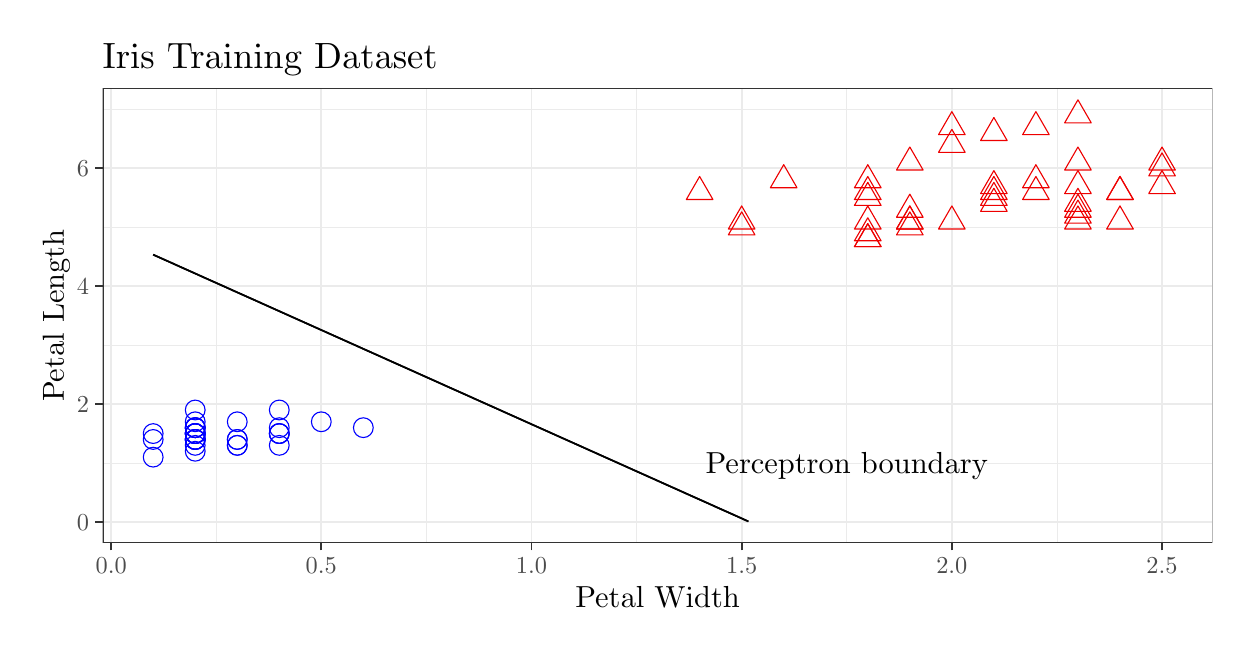
\begin{tikzpicture}[x=1pt,y=1pt]
\definecolor{fillColor}{RGB}{255,255,255}
\path[use as bounding box,fill=fillColor,fill opacity=0.00] (0,0) rectangle (433.62,216.81);
\begin{scope}
\path[clip] (  0.00,  0.00) rectangle (433.62,216.81);
\definecolor{drawColor}{RGB}{255,255,255}
\definecolor{fillColor}{RGB}{255,255,255}

\path[draw=drawColor,line width= 0.6pt,line join=round,line cap=round,fill=fillColor] (  0.00,  0.00) rectangle (433.62,216.81);
\end{scope}
\begin{scope}
\path[clip] ( 27.12, 30.72) rectangle (428.12,194.77);
\definecolor{fillColor}{RGB}{255,255,255}

\path[fill=fillColor] ( 27.12, 30.72) rectangle (428.12,194.77);
\definecolor{drawColor}{gray}{0.92}

\path[draw=drawColor,line width= 0.3pt,line join=round] ( 27.12, 59.49) --
	(428.12, 59.49);

\path[draw=drawColor,line width= 0.3pt,line join=round] ( 27.12,102.10) --
	(428.12,102.10);

\path[draw=drawColor,line width= 0.3pt,line join=round] ( 27.12,144.71) --
	(428.12,144.71);

\path[draw=drawColor,line width= 0.3pt,line join=round] ( 27.12,187.32) --
	(428.12,187.32);

\path[draw=drawColor,line width= 0.3pt,line join=round] ( 68.13, 30.72) --
	( 68.13,194.77);

\path[draw=drawColor,line width= 0.3pt,line join=round] (144.08, 30.72) --
	(144.08,194.77);

\path[draw=drawColor,line width= 0.3pt,line join=round] (220.02, 30.72) --
	(220.02,194.77);

\path[draw=drawColor,line width= 0.3pt,line join=round] (295.97, 30.72) --
	(295.97,194.77);

\path[draw=drawColor,line width= 0.3pt,line join=round] (371.92, 30.72) --
	(371.92,194.77);

\path[draw=drawColor,line width= 0.6pt,line join=round] ( 27.12, 38.18) --
	(428.12, 38.18);

\path[draw=drawColor,line width= 0.6pt,line join=round] ( 27.12, 80.79) --
	(428.12, 80.79);

\path[draw=drawColor,line width= 0.6pt,line join=round] ( 27.12,123.40) --
	(428.12,123.40);

\path[draw=drawColor,line width= 0.6pt,line join=round] ( 27.12,166.01) --
	(428.12,166.01);

\path[draw=drawColor,line width= 0.6pt,line join=round] ( 30.16, 30.72) --
	( 30.16,194.77);

\path[draw=drawColor,line width= 0.6pt,line join=round] (106.10, 30.72) --
	(106.10,194.77);

\path[draw=drawColor,line width= 0.6pt,line join=round] (182.05, 30.72) --
	(182.05,194.77);

\path[draw=drawColor,line width= 0.6pt,line join=round] (258.00, 30.72) --
	(258.00,194.77);

\path[draw=drawColor,line width= 0.6pt,line join=round] (333.95, 30.72) --
	(333.95,194.77);

\path[draw=drawColor,line width= 0.6pt,line join=round] (409.89, 30.72) --
	(409.89,194.77);
\definecolor{drawColor}{RGB}{0,0,255}

\path[draw=drawColor,line width= 0.4pt,line join=round,line cap=round] ( 60.54, 65.88) circle (  3.57);

\path[draw=drawColor,line width= 0.4pt,line join=round,line cap=round] ( 90.91, 72.27) circle (  3.57);

\path[draw=drawColor,line width= 0.4pt,line join=round,line cap=round] ( 60.54, 68.01) circle (  3.57);

\path[draw=drawColor,line width= 0.4pt,line join=round,line cap=round] ( 60.54, 68.01) circle (  3.57);
\definecolor{drawColor}{RGB}{238,0,0}

\path[draw=drawColor,line width= 0.4pt,line join=round,line cap=round] (303.57,146.00) --
	(308.37,137.67) --
	(298.76,137.67) --
	(303.57,146.00);

\path[draw=drawColor,line width= 0.4pt,line join=round,line cap=round] (303.57,167.30) --
	(308.37,158.98) --
	(298.76,158.98) --
	(303.57,167.30);
\definecolor{drawColor}{RGB}{0,0,255}

\path[draw=drawColor,line width= 0.4pt,line join=round,line cap=round] ( 60.54, 72.27) circle (  3.57);
\definecolor{drawColor}{RGB}{238,0,0}

\path[draw=drawColor,line width= 0.4pt,line join=round,line cap=round] (364.32,163.04) --
	(369.13,154.72) --
	(359.52,154.72) --
	(364.32,163.04);

\path[draw=drawColor,line width= 0.4pt,line join=round,line cap=round] (364.32,167.30) --
	(369.13,158.98) --
	(359.52,158.98) --
	(364.32,167.30);

\path[draw=drawColor,line width= 0.4pt,line join=round,line cap=round] (349.13,158.78) --
	(353.94,150.45) --
	(344.33,150.45) --
	(349.13,158.78);
\definecolor{drawColor}{RGB}{0,0,255}

\path[draw=drawColor,line width= 0.4pt,line join=round,line cap=round] ( 45.35, 70.14) circle (  3.57);
\definecolor{drawColor}{RGB}{238,0,0}

\path[draw=drawColor,line width= 0.4pt,line join=round,line cap=round] (333.95,152.39) --
	(338.75,144.06) --
	(329.14,144.06) --
	(333.95,152.39);

\path[draw=drawColor,line width= 0.4pt,line join=round,line cap=round] (379.51,152.39) --
	(384.32,144.06) --
	(374.71,144.06) --
	(379.51,152.39);
\definecolor{drawColor}{RGB}{0,0,255}

\path[draw=drawColor,line width= 0.4pt,line join=round,line cap=round] ( 75.73, 74.40) circle (  3.57);

\path[draw=drawColor,line width= 0.4pt,line join=round,line cap=round] ( 75.73, 65.88) circle (  3.57);

\path[draw=drawColor,line width= 0.4pt,line join=round,line cap=round] ( 60.54, 68.01) circle (  3.57);
\definecolor{drawColor}{RGB}{238,0,0}

\path[draw=drawColor,line width= 0.4pt,line join=round,line cap=round] (364.32,186.48) --
	(369.13,178.15) --
	(359.52,178.15) --
	(364.32,186.48);
\definecolor{drawColor}{RGB}{0,0,255}

\path[draw=drawColor,line width= 0.4pt,line join=round,line cap=round] ( 60.54, 70.14) circle (  3.57);

\path[draw=drawColor,line width= 0.4pt,line join=round,line cap=round] (121.29, 72.27) circle (  3.57);

\path[draw=drawColor,line width= 0.4pt,line join=round,line cap=round] ( 90.91, 70.14) circle (  3.57);
\definecolor{drawColor}{RGB}{238,0,0}

\path[draw=drawColor,line width= 0.4pt,line join=round,line cap=round] (394.70,163.04) --
	(399.51,154.72) --
	(389.90,154.72) --
	(394.70,163.04);

\path[draw=drawColor,line width= 0.4pt,line join=round,line cap=round] (303.57,160.91) --
	(308.37,152.59) --
	(298.76,152.59) --
	(303.57,160.91);
\definecolor{drawColor}{RGB}{0,0,255}

\path[draw=drawColor,line width= 0.4pt,line join=round,line cap=round] ( 75.73, 68.01) circle (  3.57);

\path[draw=drawColor,line width= 0.4pt,line join=round,line cap=round] ( 90.91, 65.88) circle (  3.57);

\path[draw=drawColor,line width= 0.4pt,line join=round,line cap=round] ( 60.54, 78.66) circle (  3.57);
\definecolor{drawColor}{RGB}{238,0,0}

\path[draw=drawColor,line width= 0.4pt,line join=round,line cap=round] (303.57,163.04) --
	(308.37,154.72) --
	(298.76,154.72) --
	(303.57,163.04);
\definecolor{drawColor}{RGB}{0,0,255}

\path[draw=drawColor,line width= 0.4pt,line join=round,line cap=round] ( 90.91, 70.14) circle (  3.57);
\definecolor{drawColor}{RGB}{238,0,0}

\path[draw=drawColor,line width= 0.4pt,line join=round,line cap=round] (394.70,163.04) --
	(399.51,154.72) --
	(389.90,154.72) --
	(394.70,163.04);

\path[draw=drawColor,line width= 0.4pt,line join=round,line cap=round] (318.76,150.26) --
	(323.56,141.93) --
	(313.95,141.93) --
	(318.76,150.26);
\definecolor{drawColor}{RGB}{0,0,255}

\path[draw=drawColor,line width= 0.4pt,line join=round,line cap=round] ( 60.54, 70.14) circle (  3.57);
\definecolor{drawColor}{RGB}{238,0,0}

\path[draw=drawColor,line width= 0.4pt,line join=round,line cap=round] (318.76,173.69) --
	(323.56,165.37) --
	(313.95,165.37) --
	(318.76,173.69);

\path[draw=drawColor,line width= 0.4pt,line join=round,line cap=round] (409.89,173.69) --
	(414.70,165.37) --
	(405.09,165.37) --
	(409.89,173.69);

\path[draw=drawColor,line width= 0.4pt,line join=round,line cap=round] (349.13,160.91) --
	(353.94,152.59) --
	(344.33,152.59) --
	(349.13,160.91);
\definecolor{drawColor}{RGB}{0,0,255}

\path[draw=drawColor,line width= 0.4pt,line join=round,line cap=round] ( 60.54, 68.01) circle (  3.57);
\definecolor{drawColor}{RGB}{238,0,0}

\path[draw=drawColor,line width= 0.4pt,line join=round,line cap=round] (303.57,146.00) --
	(308.37,137.67) --
	(298.76,137.67) --
	(303.57,146.00);

\path[draw=drawColor,line width= 0.4pt,line join=round,line cap=round] (258.00,150.26) --
	(262.80,141.93) --
	(253.19,141.93) --
	(258.00,150.26);
\definecolor{drawColor}{RGB}{0,0,255}

\path[draw=drawColor,line width= 0.4pt,line join=round,line cap=round] ( 75.73, 65.88) circle (  3.57);

\path[draw=drawColor,line width= 0.4pt,line join=round,line cap=round] ( 60.54, 70.14) circle (  3.57);
\definecolor{drawColor}{RGB}{238,0,0}

\path[draw=drawColor,line width= 0.4pt,line join=round,line cap=round] (379.51,154.52) --
	(384.32,146.19) --
	(374.71,146.19) --
	(379.51,154.52);

\path[draw=drawColor,line width= 0.4pt,line join=round,line cap=round] (318.76,152.39) --
	(323.56,144.06) --
	(313.95,144.06) --
	(318.76,152.39);
\definecolor{drawColor}{RGB}{0,0,255}

\path[draw=drawColor,line width= 0.4pt,line join=round,line cap=round] ( 60.54, 72.27) circle (  3.57);
\definecolor{drawColor}{RGB}{238,0,0}

\path[draw=drawColor,line width= 0.4pt,line join=round,line cap=round] (379.51,158.78) --
	(384.32,150.45) --
	(374.71,150.45) --
	(379.51,158.78);

\path[draw=drawColor,line width= 0.4pt,line join=round,line cap=round] (318.76,156.65) --
	(323.56,148.32) --
	(313.95,148.32) --
	(318.76,156.65);

\path[draw=drawColor,line width= 0.4pt,line join=round,line cap=round] (379.51,165.17) --
	(384.32,156.85) --
	(374.71,156.85) --
	(379.51,165.17);

\path[draw=drawColor,line width= 0.4pt,line join=round,line cap=round] (258.00,152.39) --
	(262.80,144.06) --
	(253.19,144.06) --
	(258.00,152.39);

\path[draw=drawColor,line width= 0.4pt,line join=round,line cap=round] (349.13,165.17) --
	(353.94,156.85) --
	(344.33,156.85) --
	(349.13,165.17);

\path[draw=drawColor,line width= 0.4pt,line join=round,line cap=round] (333.95,186.48) --
	(338.75,178.15) --
	(329.14,178.15) --
	(333.95,186.48);

\path[draw=drawColor,line width= 0.4pt,line join=round,line cap=round] (242.81,163.04) --
	(247.61,154.72) --
	(238.00,154.72) --
	(242.81,163.04);

\path[draw=drawColor,line width= 0.4pt,line join=round,line cap=round] (379.51,156.65) --
	(384.32,148.32) --
	(374.71,148.32) --
	(379.51,156.65);

\path[draw=drawColor,line width= 0.4pt,line join=round,line cap=round] (273.19,167.30) --
	(277.99,158.98) --
	(268.38,158.98) --
	(273.19,167.30);

\path[draw=drawColor,line width= 0.4pt,line join=round,line cap=round] (303.57,152.39) --
	(308.37,144.06) --
	(298.76,144.06) --
	(303.57,152.39);
\definecolor{drawColor}{RGB}{0,0,255}

\path[draw=drawColor,line width= 0.4pt,line join=round,line cap=round] ( 60.54, 68.01) circle (  3.57);

\path[draw=drawColor,line width= 0.4pt,line join=round,line cap=round] ( 60.54, 72.27) circle (  3.57);

\path[draw=drawColor,line width= 0.4pt,line join=round,line cap=round] (106.10, 74.40) circle (  3.57);

\path[draw=drawColor,line width= 0.4pt,line join=round,line cap=round] ( 45.35, 68.01) circle (  3.57);

\path[draw=drawColor,line width= 0.4pt,line join=round,line cap=round] ( 45.35, 61.62) circle (  3.57);

\path[draw=drawColor,line width= 0.4pt,line join=round,line cap=round] ( 90.91, 70.14) circle (  3.57);
\definecolor{drawColor}{RGB}{238,0,0}

\path[draw=drawColor,line width= 0.4pt,line join=round,line cap=round] (303.57,148.13) --
	(308.37,139.80) --
	(298.76,139.80) --
	(303.57,148.13);

\path[draw=drawColor,line width= 0.4pt,line join=round,line cap=round] (379.51,173.69) --
	(384.32,165.37) --
	(374.71,165.37) --
	(379.51,173.69);
\definecolor{drawColor}{RGB}{0,0,255}

\path[draw=drawColor,line width= 0.4pt,line join=round,line cap=round] ( 60.54, 74.40) circle (  3.57);

\path[draw=drawColor,line width= 0.4pt,line join=round,line cap=round] ( 60.54, 72.27) circle (  3.57);
\definecolor{drawColor}{RGB}{238,0,0}

\path[draw=drawColor,line width= 0.4pt,line join=round,line cap=round] (318.76,152.39) --
	(323.56,144.06) --
	(313.95,144.06) --
	(318.76,152.39);

\path[draw=drawColor,line width= 0.4pt,line join=round,line cap=round] (349.13,184.35) --
	(353.94,176.02) --
	(344.33,176.02) --
	(349.13,184.35);
\definecolor{drawColor}{RGB}{0,0,255}

\path[draw=drawColor,line width= 0.4pt,line join=round,line cap=round] ( 60.54, 70.14) circle (  3.57);
\definecolor{drawColor}{RGB}{238,0,0}

\path[draw=drawColor,line width= 0.4pt,line join=round,line cap=round] (409.89,165.17) --
	(414.70,156.85) --
	(405.09,156.85) --
	(409.89,165.17);
\definecolor{drawColor}{RGB}{0,0,255}

\path[draw=drawColor,line width= 0.4pt,line join=round,line cap=round] ( 75.73, 68.01) circle (  3.57);

\path[draw=drawColor,line width= 0.4pt,line join=round,line cap=round] ( 60.54, 70.14) circle (  3.57);
\definecolor{drawColor}{RGB}{238,0,0}

\path[draw=drawColor,line width= 0.4pt,line join=round,line cap=round] (394.70,152.39) --
	(399.51,144.06) --
	(389.90,144.06) --
	(394.70,152.39);
\definecolor{drawColor}{RGB}{0,0,255}

\path[draw=drawColor,line width= 0.4pt,line join=round,line cap=round] ( 90.91, 78.66) circle (  3.57);
\definecolor{drawColor}{RGB}{238,0,0}

\path[draw=drawColor,line width= 0.4pt,line join=round,line cap=round] (333.95,180.08) --
	(338.75,171.76) --
	(329.14,171.76) --
	(333.95,180.08);

\path[draw=drawColor,line width= 0.4pt,line join=round,line cap=round] (379.51,190.74) --
	(384.32,182.41) --
	(374.71,182.41) --
	(379.51,190.74);

\path[draw=drawColor,line width= 0.4pt,line join=round,line cap=round] (409.89,171.56) --
	(414.70,163.24) --
	(405.09,163.24) --
	(409.89,171.56);
\definecolor{drawColor}{RGB}{0,0,255}

\path[draw=drawColor,line width= 0.4pt,line join=round,line cap=round] ( 60.54, 63.75) circle (  3.57);
\definecolor{drawColor}{RGB}{238,0,0}

\path[draw=drawColor,line width= 0.4pt,line join=round,line cap=round] (349.13,163.04) --
	(353.94,154.72) --
	(344.33,154.72) --
	(349.13,163.04);
\definecolor{drawColor}{RGB}{0,0,255}

\path[draw=drawColor,line width= 0.4pt,line join=round,line cap=round] ( 60.54, 70.14) circle (  3.57);
\definecolor{drawColor}{RGB}{0,0,0}

\path[draw=drawColor,line width= 0.6pt,line join=round] ( 45.35,134.78) --
	( 48.99,133.15) --
	( 52.64,131.52) --
	( 56.28,129.88) --
	( 59.93,128.25) --
	( 63.57,126.61) --
	( 67.22,124.98) --
	( 70.86,123.35) --
	( 74.51,121.71) --
	( 78.16,120.08) --
	( 81.80,118.45) --
	( 85.45,116.81) --
	( 89.09,115.18) --
	( 92.74,113.54) --
	( 96.38,111.91) --
	(100.03,110.28) --
	(103.67,108.64) --
	(107.32,107.01) --
	(110.96,105.38) --
	(114.61,103.74) --
	(118.26,102.11) --
	(121.90,100.47) --
	(125.55, 98.84) --
	(129.19, 97.21) --
	(132.84, 95.57) --
	(136.48, 93.94) --
	(140.13, 92.31) --
	(143.77, 90.67) --
	(147.42, 89.04) --
	(151.06, 87.40) --
	(154.71, 85.77) --
	(158.36, 84.14) --
	(162.00, 82.50) --
	(165.65, 80.87) --
	(169.29, 79.24) --
	(172.94, 77.60) --
	(176.58, 75.97) --
	(180.23, 74.33) --
	(183.87, 72.70) --
	(187.52, 71.07) --
	(191.16, 69.43) --
	(194.81, 67.80) --
	(198.46, 66.17) --
	(202.10, 64.53) --
	(205.75, 62.90) --
	(209.39, 61.26) --
	(213.04, 59.63) --
	(216.68, 58.00) --
	(220.33, 56.36) --
	(223.97, 54.73) --
	(227.62, 53.10) --
	(231.26, 51.46) --
	(234.91, 49.83) --
	(238.56, 48.19) --
	(242.20, 46.56) --
	(245.85, 44.93) --
	(249.49, 43.29) --
	(253.14, 41.66) --
	(256.78, 40.03) --
	(260.43, 38.39);

\path[draw=drawColor,line width= 0.6pt,line join=round] ( 45.35,134.78) --
	( 48.99,133.15) --
	( 52.64,131.52) --
	( 56.28,129.88) --
	( 59.93,128.25) --
	( 63.57,126.61) --
	( 67.22,124.98) --
	( 70.86,123.35) --
	( 74.51,121.71) --
	( 78.16,120.08) --
	( 81.80,118.45) --
	( 85.45,116.81) --
	( 89.09,115.18) --
	( 92.74,113.54) --
	( 96.38,111.91) --
	(100.03,110.28) --
	(103.67,108.64) --
	(107.32,107.01) --
	(110.96,105.38) --
	(114.61,103.74) --
	(118.26,102.11) --
	(121.90,100.47) --
	(125.55, 98.84) --
	(129.19, 97.21) --
	(132.84, 95.57) --
	(136.48, 93.94) --
	(140.13, 92.31) --
	(143.77, 90.67) --
	(147.42, 89.04) --
	(151.06, 87.40) --
	(154.71, 85.77) --
	(158.36, 84.14) --
	(162.00, 82.50) --
	(165.65, 80.87) --
	(169.29, 79.24) --
	(172.94, 77.60) --
	(176.58, 75.97) --
	(180.23, 74.33) --
	(183.87, 72.70) --
	(187.52, 71.07) --
	(191.16, 69.43) --
	(194.81, 67.80) --
	(198.46, 66.17) --
	(202.10, 64.53) --
	(205.75, 62.90) --
	(209.39, 61.26) --
	(213.04, 59.63) --
	(216.68, 58.00) --
	(220.33, 56.36) --
	(223.97, 54.73) --
	(227.62, 53.10) --
	(231.26, 51.46) --
	(234.91, 49.83) --
	(238.56, 48.19) --
	(242.20, 46.56) --
	(245.85, 44.93) --
	(249.49, 43.29) --
	(253.14, 41.66) --
	(256.78, 40.03) --
	(260.43, 38.39);

\node[text=drawColor,anchor=base,inner sep=0pt, outer sep=0pt, scale=  1.10] at (295.97, 55.68) {Perceptron boundary};
\definecolor{drawColor}{gray}{0.20}

\path[draw=drawColor,line width= 0.6pt,line join=round,line cap=round] ( 27.12, 30.72) rectangle (428.12,194.77);
\end{scope}
\begin{scope}
\path[clip] (  0.00,  0.00) rectangle (433.62,216.81);
\definecolor{drawColor}{gray}{0.30}

\node[text=drawColor,anchor=base east,inner sep=0pt, outer sep=0pt, scale=  0.88] at ( 22.17, 35.15) {0};

\node[text=drawColor,anchor=base east,inner sep=0pt, outer sep=0pt, scale=  0.88] at ( 22.17, 77.76) {2};

\node[text=drawColor,anchor=base east,inner sep=0pt, outer sep=0pt, scale=  0.88] at ( 22.17,120.37) {4};

\node[text=drawColor,anchor=base east,inner sep=0pt, outer sep=0pt, scale=  0.88] at ( 22.17,162.98) {6};
\end{scope}
\begin{scope}
\path[clip] (  0.00,  0.00) rectangle (433.62,216.81);
\definecolor{drawColor}{gray}{0.20}

\path[draw=drawColor,line width= 0.6pt,line join=round] ( 24.37, 38.18) --
	( 27.12, 38.18);

\path[draw=drawColor,line width= 0.6pt,line join=round] ( 24.37, 80.79) --
	( 27.12, 80.79);

\path[draw=drawColor,line width= 0.6pt,line join=round] ( 24.37,123.40) --
	( 27.12,123.40);

\path[draw=drawColor,line width= 0.6pt,line join=round] ( 24.37,166.01) --
	( 27.12,166.01);
\end{scope}
\begin{scope}
\path[clip] (  0.00,  0.00) rectangle (433.62,216.81);
\definecolor{drawColor}{gray}{0.20}

\path[draw=drawColor,line width= 0.6pt,line join=round] ( 30.16, 27.97) --
	( 30.16, 30.72);

\path[draw=drawColor,line width= 0.6pt,line join=round] (106.10, 27.97) --
	(106.10, 30.72);

\path[draw=drawColor,line width= 0.6pt,line join=round] (182.05, 27.97) --
	(182.05, 30.72);

\path[draw=drawColor,line width= 0.6pt,line join=round] (258.00, 27.97) --
	(258.00, 30.72);

\path[draw=drawColor,line width= 0.6pt,line join=round] (333.95, 27.97) --
	(333.95, 30.72);

\path[draw=drawColor,line width= 0.6pt,line join=round] (409.89, 27.97) --
	(409.89, 30.72);
\end{scope}
\begin{scope}
\path[clip] (  0.00,  0.00) rectangle (433.62,216.81);
\definecolor{drawColor}{gray}{0.30}

\node[text=drawColor,anchor=base,inner sep=0pt, outer sep=0pt, scale=  0.88] at ( 30.16, 19.71) {0.0};

\node[text=drawColor,anchor=base,inner sep=0pt, outer sep=0pt, scale=  0.88] at (106.10, 19.71) {0.5};

\node[text=drawColor,anchor=base,inner sep=0pt, outer sep=0pt, scale=  0.88] at (182.05, 19.71) {1.0};

\node[text=drawColor,anchor=base,inner sep=0pt, outer sep=0pt, scale=  0.88] at (258.00, 19.71) {1.5};

\node[text=drawColor,anchor=base,inner sep=0pt, outer sep=0pt, scale=  0.88] at (333.95, 19.71) {2.0};

\node[text=drawColor,anchor=base,inner sep=0pt, outer sep=0pt, scale=  0.88] at (409.89, 19.71) {2.5};
\end{scope}
\begin{scope}
\path[clip] (  0.00,  0.00) rectangle (433.62,216.81);
\definecolor{drawColor}{RGB}{0,0,0}

\node[text=drawColor,anchor=base,inner sep=0pt, outer sep=0pt, scale=  1.10] at (227.62,  7.44) {Petal Width};
\end{scope}
\begin{scope}
\path[clip] (  0.00,  0.00) rectangle (433.62,216.81);
\definecolor{drawColor}{RGB}{0,0,0}

\node[text=drawColor,rotate= 90.00,anchor=base,inner sep=0pt, outer sep=0pt, scale=  1.10] at ( 13.08,112.75) {Petal Length};
\end{scope}
\begin{scope}
\path[clip] (  0.00,  0.00) rectangle (433.62,216.81);
\definecolor{drawColor}{RGB}{0,0,0}

\node[text=drawColor,anchor=base west,inner sep=0pt, outer sep=0pt, scale=  1.32] at ( 27.12,202.22) {Iris Training Dataset};
\end{scope}
\end{tikzpicture}
